\documentclass[10pt, landscape]{article}
\usepackage[scaled=0.92]{helvet}
\usepackage{calc}
\usepackage{multicol}
\usepackage{ifthen}
\usepackage[a4paper,margin=5mm,landscape]{geometry}
\usepackage{amsmath,amsthm,amsfonts,amssymb}
\usepackage{color,graphicx,overpic}
\usepackage{hyperref}
\usepackage{newtxtext} 
\usepackage{enumitem}
\usepackage{amssymb}
\usepackage[table]{xcolor}
\usepackage{vwcol}
\usepackage{tikz}
\usetikzlibrary{arrows.meta}
\usetikzlibrary{calc}
\usepackage{mathtools}
\usepackage{nicematrix}
\usepackage[T1]{fontenc} %%% <--- NOTE THIS
% for relations
\usepackage{cancel}
\usepackage{ mathrsfs }
\usepackage{listings}
\usepackage{background}
\setlist{nosep}

\usepackage{etoolbox}
\makeatletter
\preto{\@verbatim}{\topsep=0pt \partopsep=0pt }
\makeatother

\backgroundsetup{
scale=1,
color=black,
opacity=0.3,
angle=0,
contents={}
% {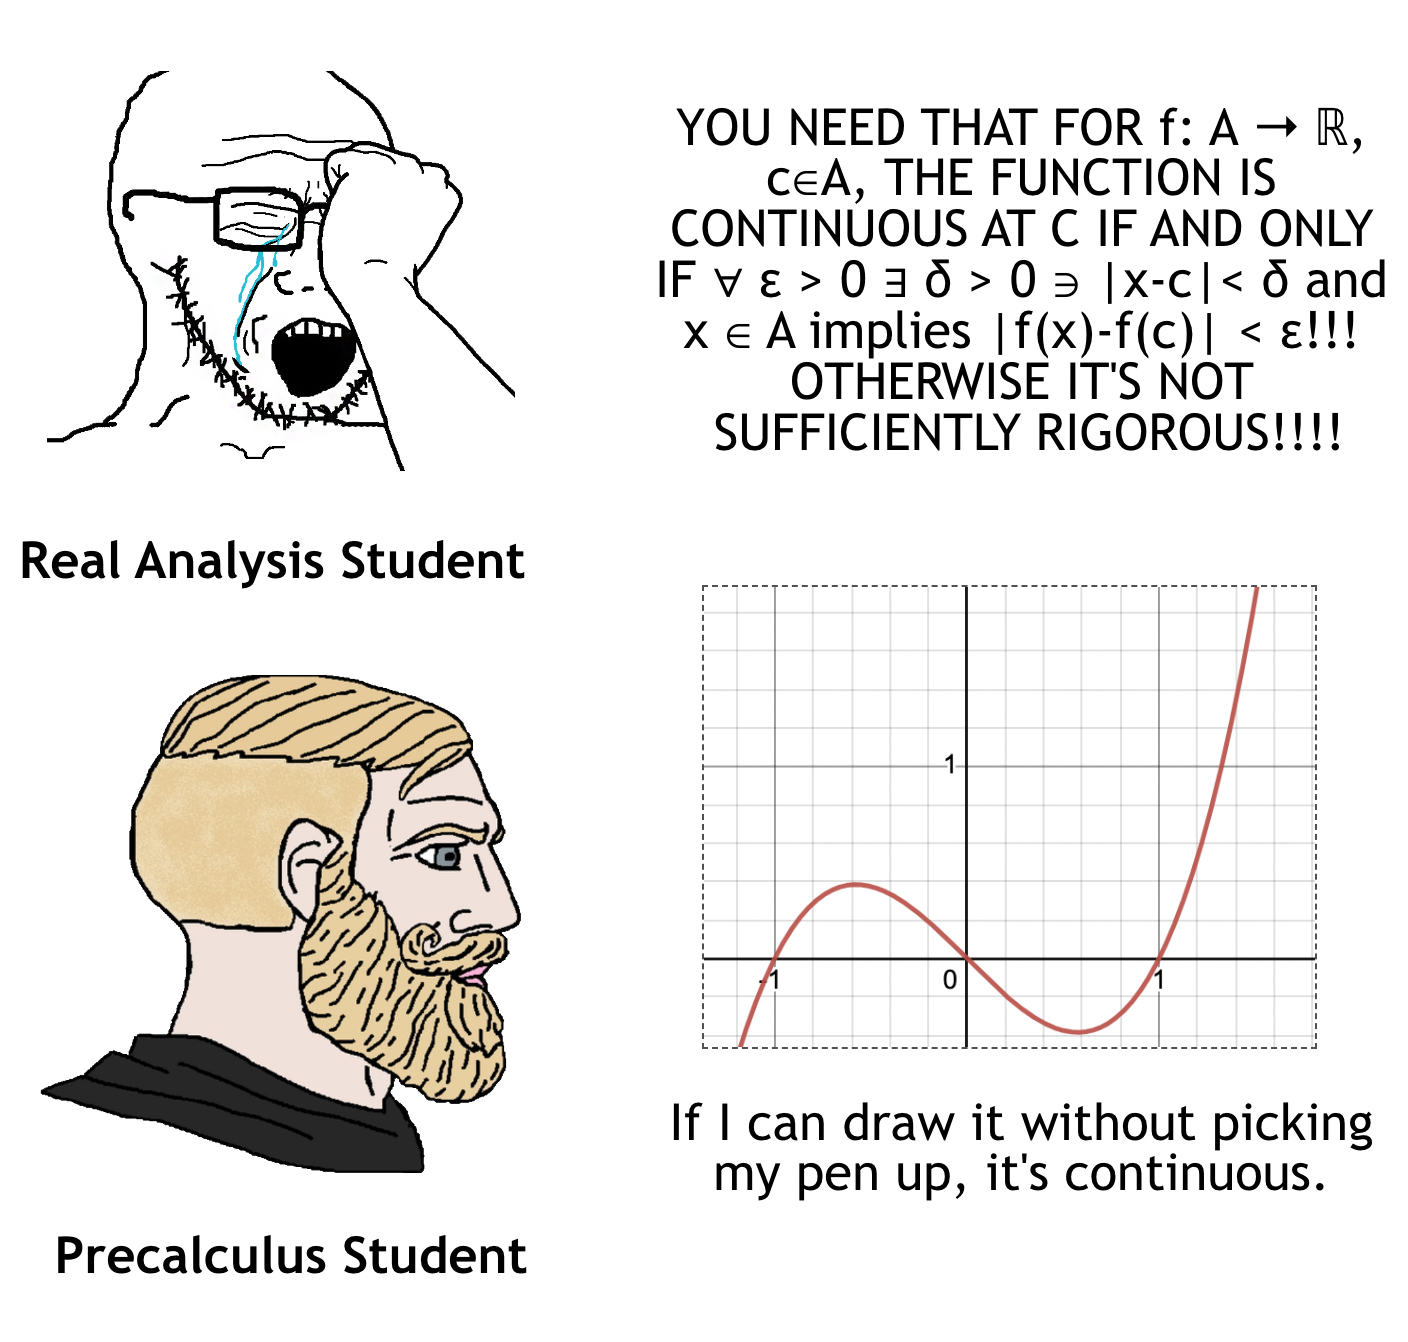
\includegraphics[width=\paperwidth,height=\paperheight]{meme.png}}
}

\pdfinfo{
  /Title (MA2108.pdf)
  /Creator (TeX)
  /Producer (pdfTeX 1.40.0)
  /Author (Seamus)
  /Subject (Example)
  /Keywords (pdflatex, latex,pdftex,tex)}

\lstset{language=Java,keywordstyle={\bfseries \color{black}}}

% Turn off header and footer
\pagestyle{empty}

\newenvironment{tightcenter}{%
  \setlength\topsep{0pt}
  \setlength\parskip{0pt}
  \begin{center}
}{%
  \end{center}
}

% redefine section commands to use less space
\makeatletter
\renewcommand{\section}{\@startsection{section}{1}{0mm}%
                                {-1ex plus -.5ex minus -.2ex}%
                                {0.5ex plus .2ex}%x
                                {\normalfont\large\bfseries}}
\renewcommand{\section}{\@startsection{section}{2}{0mm}%
                                {-1explus -.5ex minus -.2ex}%
                                {0.5ex plus .2ex}%
                                {\normalfont\normalsize\bfseries}}
\renewcommand{\subsection}{\@startsection{subsection}{3}{0mm}%
                                {-1ex plus -.5ex minus -.2ex}%
                                {1ex plus .2ex}%
                                {\normalfont\small\bfseries}}%
\renewcommand{\familydefault}{\sfdefault}
\renewcommand\rmdefault{\sfdefault}
% makes nested numbering (e.g. 1.1.1, 1.1.2, etc)
\renewcommand{\labelenumii}{\theenumii}
\renewcommand{\theenumii}{\theenumi.\arabic{enumii}.}
\renewcommand\labelitemii{•}
%  for logical not operator
\renewcommand{\lnot}{\mathord{\sim}}
\renewcommand{\bf}[1]{\textbf{#1}}
\newcommand{\abs}[1]{\vert #1 \vert}
\newcommand{\Mod}[1]{\ \mathrm{mod}\ #1}

\makeatother
\definecolor{myblue}{cmyk}{1,.72,0,.38}
\everymath\expandafter{\the\everymath \color{myblue}}
% Define BibTeX command
\def\BibTeX{{\rm B\kern-.05em{\sc i\kern-.025em b}\kern-.08em
    T\kern-.1667em\lower.7ex\hbox{E}\kern-.125emX}}
\let\iff\leftrightarrow
\let\Iff\Leftrightarrow
\let\then\rightarrow
\let\Then\Rightarrow

% Don't print section numbers
\setcounter{secnumdepth}{0}

\setlength{\parindent}{0pt}
\setlength{\parskip}{0pt plus 0.5ex}
%% this changes all items (enumerate and itemize)
\setlength{\leftmargini}{0.5cm}
\setlength{\leftmarginii}{0.5cm}
\setlist[itemize,1]{leftmargin=2mm,labelindent=1mm,labelsep=1mm}
\setlist[itemize,2]{leftmargin=4mm,labelindent=1mm,labelsep=1mm}

%My Environments
\newtheorem{example}[section]{Example}
% -----------------------------------------------------------------------

\begin{document}
\raggedright
\footnotesize
\begin{multicols*}{3}

% multicol parameters
% These lengths are set only within the two main columns
\setlength{\columnseprule}{0.25pt}
\setlength{\premulticols}{1pt}
\setlength{\postmulticols}{1pt}
\setlength{\multicolsep}{1pt}
\setlength{\columnsep}{2pt}

\begin{center}
    \fbox{%
        \parbox{0.8\linewidth}{\centering \textcolor{black}{
            {\Large\textbf{MA2108}}
            \\ \normalsize{AY25/26 Sem 1}}
            \\ {\footnotesize \textcolor{myblue}{by ngmh}} 
        }%
    }
\end{center}

\section{Ordered Fields}
\textbf{D1.1 Field} A field is a set $F$ with addition and multiplication. $\mathbb{R}, \mathbb{Q}$ are fields while $\mathbb{N}, \mathbb{Z}$ are not.

\textbf{Addition Axioms} Closure of Addition, Commutativity, Associativity, Identity Element, Additive Inverse

\textbf{Multiplication Axioms} Closure of Multiplication, Commutativity, Associativity, Identity Element, Multiplicative Inverse, Distributive Law

\textbf{P1.4}
\begin{itemize}
    \item $x+y=x+z \Rightarrow y = z$
    \item $x+y=x \Rightarrow y = 0$
    \item $x+y = 0 \Rightarrow y = -x$
    \item $-(-x)=x$
    \item $x \neq 0 \land xy = xz \Rightarrow y  = z$
    \item $x \neq 0 \land xy = x \Rightarrow y = 1$
    \item $x \neq 0 \land xy = 1 \Rightarrow y = 1/x$
    \item $x \neq 0 \Rightarrow1/(1/x) = x$
    \item $0x = 0$
    \item $x \neq 0 \land y \neq 0 \Rightarrow xy \neq 0$
    \item $(-x)y=-(xy)=x(-y)$
    \item $(-x)(-y)=xy$
\end{itemize}

\textbf{D1.5 Total Order} A relation satisfying trichotomy and transitivity property. An ordered set is a set with a total order.

\textbf{D1.8 Ordered Field} A field where $y < z \Rightarrow x+y<x+z$, $x>0, y>0 \Rightarrow xy > 0$. All ordered fields contain (a homomorphism of) $\mathbb{Q}$.

\textbf{P1.12 Ordered Field Statements}
\begin{itemize}
    \item $x>0 \Rightarrow -x < 0$ and vice versa
    \item $x > 0 \land y < z \Rightarrow xy<xz$
    \item $x<0 \land y<z \Rightarrow xy > xz$
    \item $xy>0 \Rightarrow (x > 0 \land y>0) \lor (x<0 \land y<0)$
    \item $x \neq 0 \Rightarrow x^2>0$
    \item $0<x<y \Rightarrow 0< 1/y < 1/x$
\end{itemize}

\textbf{P1.15} There exists $\iota : \mathbb{Q} \hookrightarrow F$ such that $\iota$ is order preserving for all ordered fields.

\section{Least Upper Bound Property}
\textbf{D1.16 Upper Bound} Suppose $S$ is an ordered set and $E \subset S$. If $\exists \beta \in S, \forall x \in E, x \leq \beta \ $, then $E$ is bounded above and $\beta$ is an upper bound of $E$. Lower bound is defined similarly with $\geq$. They might not be unique and could possibly not exist. They might not be in the set itself.

\textbf{D1.19 Least Upper Bound} Suppose $\alpha \in S$, $\alpha$ is an upper bound of $E$, and if $\gamma < \alpha$ then $\gamma$ is not an upper bound of $E$. Then $\alpha$ is the least upper bound or supremum of $E$, and $\alpha = sup\ E$. We can similarly define the greatest lower bound or infimum $\alpha = inf \ E$. The LUB is also unique.

\textbf{R1.20 Maximum} $\alpha$ is a maximum of $E$ if it is a LUB and $\alpha \in E$.

\textbf{T1.26 Least Upper Bound Property} An ordered set $S$ where $\forall E \subseteq S, E \neq \emptyset,$ and $E$ is bounded above implies $\exists sup\ E \in S$. $\mathbb{Q}$ does not have this property.

\textbf{T1.29 Completeness of $\mathbb{R}$} $\mathbb{R}$ is the ordered field which has the LUB property and is unique up to isomorphism. It also contains $\mathbb{Q}$ as a subfield.

\textbf{T1.32} An ordered set with the LUB property also has the GLB property.

\textbf{P1.34} Let $E \subset \mathbb{R}, a \in \mathbb{R}, T=\{a+x:x\in E\}$. If $E$ is bounded above, then $sup\ T=a+sup\ E$.
\begin{itemize}
    \item $\emptyset \neq E \subseteq \mathbb{R}$, $E$ is bounded above, so $sup\ E$ exists
    \item $\forall x \in E, x \leq sup\ E, a+x \leq a + sup\ E$
    \item $a+sup\ E$ must be an upper bound for $T$, let $M$ be any upper bound of $T$
    \item $\forall x \in E, a+x \leq M, x \leq M-a$
    \item $M-a$ is an upper bound for $E$
    \item By definition of supremum, $sup\ E \leq M-a, a+sup\ E \leq M, sup\ T \geq a + sup\ E$
\end{itemize}

\textbf{R1.35} To show equality, either show $A \leq B \land B \leq A$ or $A \leq B$, $A<B$ is a contradiction

\section{Archimedean Property}
\textbf{D2.1 Archimedean Property} Let $F$ be an ordered field. $F$ has the Archimedean Property if $\forall a,b \in F, a > 0, \exists n \in \mathbb{N}, na > b \in F$

\textbf{D2.1 Density} For an ordered field $F$, $\mathbb{Q}$ is dense in $F$ wrt ordering if $\forall x, y \in F, x<y, \exists r \in \mathbb{Q}, x < r < y \in F$

\textbf{P2.4} $F$ has the Archimedean Property iff $\mathbb{Q}$ is dense in $F$

\textbf{$\mathbb{Q}, \mathbb{R}$:} $\mathbb{Q}$ is Archimedean and is dense in itself, while $\mathbb{R}$ is Archimedean as well

\textbf{C2.6} $\forall \varepsilon \in \mathbb{R}_{>0}, \exists\ n \in \mathbb{N}, 0 < \frac{1}{n} < \varepsilon$

\textbf{T2.7 nth roots} $\forall x \in  \mathbb{R}_{>0}, n > 0 \in \mathbb{Z}, \exists!\ y, y^n = x$

\textbf{C2.8} For positive real $a,b$ and positive integer $n$, $(ab)^{1/n}=a^{1/n}b^{1/n}$

\textbf{C2.9} If $a,b \in \mathbb{R}, a<b, \exists \ x \in \mathbb{R} \backslash \mathbb{Q}, a<x<b$

\textbf{P2.10} Let $\alpha \in \mathbb{R}, E=\{x \in \mathbb{Q}: x < \alpha\} \subseteq \mathbb{Q}$. Then $sup \ E = \alpha$

\section{Sequences}
\textbf{P2.13 Properties of absolute value}
\begin{itemize}
    \item $|a| \geq 0, a \leq |a|, -a \leq |a|$
    \item $|a|=0 \Leftrightarrow a = 0$
    \item $|-a|=|a|$
    \item $|ab|=|a|\cdot |b|$
    \item $|a|^2=a^2$
    \item $c \geq 0 \Rightarrow |a| \leq c \Leftrightarrow -c \leq a \leq c$
    \item $-|a| \leq a \leq |a|$
\end{itemize}

\textbf{P2.14 Triangle Inequality} $\forall a, b \in F, |a+b| \leq |a|+|b|$

\textbf{C2.15} $\forall a, b \in F$,
\begin{itemize}
    \item $||a|-|b|| \leq |a-b|$
    \item $|a-b| \leq |a|+|b|$
    \item $||a|-|b|| \leq |a+b|$
\end{itemize}

\textbf{D2.16 Sequences} A sequence in a set $X$ is a function $x:\mathbb{N}\rightarrow X$, denoted by $(x_n)_n$ or $\{x_n\}_n$.

\textbf{D2.21 Convergence} A sequence in $F$ converges iff $\exists x \in F, \forall \varepsilon \in F_{>0}, \exists N \in \mathbb{N}, \forall n \in \mathbb{N}, n \geq N \Rightarrow |x_n-x| < \varepsilon$. For every small distance $\varepsilon$, there is a cut-off $N$ such that for all larger $n$, the absolute difference is smaller than $\varepsilon$. $x$ is the limit of the sequence in $F$, and $lim_{n\rightarrow\infty}x_n=x$.

\textbf{P2.23} The limit of a sequence is unique.

\textbf{D2.24 Bounds} A sequence is eventually constant if $\exists N \in \mathbb{N}, \forall n \geq N, x_n=x_N=x$. A sequence is bounded in $F$ if the set of values is bounded in $F$ by some $B$. We can define one sided bounds similarly.

\textbf{P2.26} If a sequence is convergent in $F$, then it is bounded.

\textbf{E2.29} Example Convergence Proof (Make $n$ subject of formula)
\begin{align*} 
\left|\frac{2n^2+1}{n^2+3n}-2\right|&=\left|\frac{2n^2+1-2(n^2+3n)}{n^2+3n}\right|\\
&=\left|\frac{1-6n}{n^2+3n}\right|\\
&\leq \frac{1+6n}{n^2+3n}\\
&\leq \frac{n+6n}{n^2}=\frac{7n}{n^2}=\frac{7}{n}
\end{align*}
\begin{itemize}
    \item Let $\varepsilon > 0$ be given, then choose $K\in \mathbb{N}$ such that $K  > \frac{7}{\varepsilon}$. Then $\forall n \geq K$,
\end{itemize}
\begin{align*}
\left|\frac{2n^2+1}{n^2+3n}-2\right|&\leq \frac{7}{n} \text{ since $n \geq K$}\\
&\leq\frac{7}{K}\\
&<\varepsilon \text{ since $K > \frac{7}{\varepsilon}$}
\end{align*}

\section{Convergent Sequences}
\textbf{P3.1 Properties of Limits of Convergent Sequences} Let $(s_n)_n, (t_n)_n$ be convergent sequences in $F$. Then $(s_n+t_n)_n, (cs_n)_n, (s_nt_n)_n, (|s_n|)_n, (\sqrt{s_n})_n, (\frac{1}{s_n})_n$ are all convergent with limits following the substitution. If $\exists N \in \mathbb{N}, \forall n \geq N, s_n \leq t_n$, then $lim_{n\rightarrow\infty}s_n \leq lim_{n\rightarrow \infty}t_n$.

\textbf{P3.2 Squeeze Theorem} If $(x_n)_n, (y_n)_n, (z_n)_n$ are sequences in an ordered field $F$ such that $\forall n, x_n \leq y_n \leq z_n$ and $lim_{n\rightarrow\infty}x_n=lim_{n\rightarrow\infty}z_n=a$, then $lim_{n\rightarrow\infty}y_n=a$.

\section{More Sequences}
\textbf{E3.3} For real $0 \leq b < 1$, $lim_{n\rightarrow\infty}b^n=0$.

\textbf{E3.6} For real $c > 0$, $lim_{n\rightarrow\infty}c^{\frac{1}{n}}=1$.

\textbf{E3.7} For real $a>1$ and integer $k>0$, $lim_{n\rightarrow\infty}\frac{n^k}{a^n}=0$.

\textbf{E3.8} $lim_{n \rightarrow \infty} n^{\frac{1}{n}} = 1$

\textbf{D3.9 Monotone Sequences} $(s_n)$ is monotonically increasing if $\forall n,s_n \leq s_{n+1}$, while it is monotonically decreasing if $\forall n, s_n \geq s_{n+1}$.

\textbf{T3.10 Monotone Convergence} Every monotone sequence in $\mathbb{R}$ is bounded iff it converges.

\section{Subsequences, Cauchy Sequences}
\textbf{D4.2 Subsequence} Given a sequence in $F$, consider $(n_k)_k$ of positive integers where $n_1<n_2<...<n_k<...$. Then $(x_{n_k})_k$ is a subsequence of $(x_n)_n$.

\textbf{E4.3} A sequence converges to $x$ iff every subsequence also converges to $x$.

\textbf{R4.5} For divergence, we can show a subsequence which diverges, or two subsequences which converge to different limits.

\textbf{T4.9 Existence of Monotone Subsequence} Let there be a sequence in an ordered field $F$ which is not necessarily convergent. There exists a monotone subsequence in it.

\textbf{T4.10 Bolzano-Weierstrass} Every bounded sequence in $\mathbb{R}$ has a convergent subsequence.

\textbf{D4.11 Cauchy Sequence} A sequence $(p_n)_n$ in $F$ is said to be Cauchy if $\forall \varepsilon \in F_{>0}, \exists N \in \mathbb{N}, \forall m,n \in \mathbb{N}_{\geq N}, |p_n-p_m|<\varepsilon$.

\textbf{P4.13} If a sequence is convergent, then it is Cauchy.

\textbf{P4.15} If a sequence is Cauchy, then it is bounded.

\textbf{P4.16 Properties of Cauchy Sequences} If $(s_n),(t_n)$ are Cauchy sequences, then $(s_n+t_n), (cs_n), (s_nt_n), (|s_n|)$ are also Cauchy.

\section{More Cauchy Sequences}
\textbf{D4.18 Cauchy Complete} An ordered field in $F$ is Cauchy complete iff every Cauchy sequence in $F$ is convergent in 
$F$. $\mathbb{R}$ is Cauchy complete.

\textbf{P4.19} Let $p_n$ be a Cauchy sequence in $F$. If there exists a subsequence of $p_n$ that converges in $F$, then $p_n$ also converges in $F$ to the same limit.

\textbf{T4.20} $\mathbb{R}$ is Cauchy complete.

\textbf{D4.22 Contractive} A sequence $x_n$ is contractive if there exists $C$ with $0<C<1$ such that $|x_{n+2}-x_{n+1}|\leq C|x_{n+1}-x_n|$ where $C$ does not depend on $n$.

\textbf{P4.23} Every contractive sequence is Cauchy and thus convergent.

\textbf{D4.24 Extended Real Numbers} The extended real number system consists of $\mathbb{R}$, $+\infty$, and $-\infty$. The original order is preserved and $\forall x \in \mathbb{R}, -\infty < x < +\infty$. This ordered set (not field) is denoted by $[-\infty, +\infty]$. The supremum and infimum of any subset always exists.

\textbf{D4.28 Limit to Infinity} The limit of $x_n$ is $+\infty$ if for all real $M, \exists N, \forall n \geq N, s_n \geq M$. Similarly for $-\infty$.

\textbf{P4.30} Let $x_n$ be a sequence in $\mathbb{R}$, $x \in [-\infty, +\infty]$. Then $x_n \rightarrow x $ iff $\forall A \in [-\infty, \infty], A < x, \exists N \in \mathbb{N}, \forall n \in \mathbb{N}, n \geq N \Rightarrow A<x_n$ and the opposite holds.

\textbf{L4.31} For any sequence $x_n\in\mathbb{R}$, there exists a subsequence $x_{n_i}$ which converges in $[-\infty, +\infty]$.

\section{limsup, liminf}
\textbf{D5.1 limsup, liminf} Let $x_n$ be a sequence in $\mathbb{R}$. Let $E=\{\text{the limits in $[-\infty, +\infty]$ of all convergent subsequences of $x_n$}\}$. Then define $\limsup_{n \rightarrow \infty}=sup(E), \liminf_{n\rightarrow\infty}=inf(E)$. $\limsup$ is the limit superior, while $\liminf$ is the limit inferior.

\textbf{P5.3 Equivalent Definition} Let $x_n$ be a bounded series in $\mathbb{R}$ and $M=\limsup x_n$. $M=\limsup x_n$ if $M\in\mathbb{R}$ satisfies the following: For each $\varepsilon>0$ there are at most finitely many $n$ such that $x_n \geq M + \varepsilon$. Alternatively, $\forall\varepsilon, \exists K\in\mathbb{N}, \forall n \geq K, x_n < M + \varepsilon$. Also, for each $\varepsilon>0$, there are infinitely many $n$ such that $x_n > M-\varepsilon$. The same holds for $\liminf$.

\textbf{P5.5 Convergence with limsup, liminf} Let $s_n$ be a sequence in $\mathbb{R}$. Then $\liminf _{n \rightarrow\infty} s_n \leq \limsup_{n \rightarrow\infty} s_n \in [-\infty, +\infty]$. Equality only holds iff $s_n$ converges.

\textbf{P5.7} If $s_n \leq t_n, \forall n \geq N$, $\liminf_{n\rightarrow\infty}s_n \leq\liminf_{n\rightarrow\infty}t_n$ and $\limsup_{n\rightarrow\infty}s_n \leq \limsup_{n\rightarrow\infty}t_n$

\textbf{P5.8 Equivalent Definition of limsup} Let $x_n$ be a bounded sequence. For each $n \in \mathbb{N}$, let $y_n=sup\{x_k:k\geq n\}$. Then $\limsup_{n\rightarrow\infty}x_n=lim_{n \rightarrow\infty}y_n$.

\textbf{P5.9 Equivalent Definition of liminf} Let $x_n$ be a bounded sequence. For each $n \in \mathbb{N}$, let $z_n=inf\{x_k:k\geq n\}$. Then $z_n$ is increasing and bounded and $\liminf x_n=lim_{n\rightarrow\infty}z_n$

\section{Series}
\textbf{D5.10 Series} Let $F$ be an ordered field. Given a sequence $a_n\in F$, we can form an infinite series $\sum_{k=1}^\infty a_k=a_1+a_2+...$. More precisely, define $S_k=\sum_{n=1}^ka_n$ (nth partial sum).

\textbf{P5.13 Properties of Convergent Series} If $\sum a_n, \sum b_n$ are convergent series and $c \in F$, then $\sum(a_n+b_n),$ and $\sum ca_n$ are convergent.

\textbf{P5.14 Cauchy Criterion for Series} Let $a_n$ be a sequence in $\mathbb{R}$. Then $\sum a_n$ converges iff $\forall \varepsilon>0, \exists N,\forall m,n, m \geq n \geq N,|\sum_{k=n}^ma_k|\leq \varepsilon$.

\textbf{C5.15} If $\sum a_n$ converges, $lim_{n\rightarrow\infty}a_n=0$. However, the converse is false.

\textbf{C5.17 nth term test} If $a_n$ does not converge or converges to a nonzero, then $\sum a_n$ diverges.

\textbf{D5.19} A series eventually has a property (*) if $\exists N \in \mathbb{N}, \forall k \geq N, a_k$ has (*).

\textbf{P5.20} Let $\sum a_n$ be an eventually non-negative series where $a_n \in \mathbb{R}$. Then $a_n$ converges iff $S_n$ is bounded above.

\textbf{E5.21 Geometric Series} For $\sum_{k=1}^\infty ar^{k-1}$, $s_n=\frac{a(1-r^n)}{1-r}$ if $r \neq 1$.

\textbf{E5.22 p-series} If $p>1$, the p-series $\sum \frac{1}{n^p}$ converges. When $p \leq 1$, the series diverges.

\textbf{D5.23 Absolute Convergence} The series $\sum a_n$ converges absolutely if $\sum |a_n|$ converges. If a series converges but not absolutely, it converges conditionally.

\textbf{P5.24} Let $a_n$ be a sequence in $\mathbb{R}$. If $\sum a_n$ converges absolutely, then $a_n$ converges. However, the converse is false.

\section{Convergence Tests}
\textbf{P6.1 Direct Comparison Test} Let $a_k, b_k$ be sequences in $\mathbb{R}$ such that $\sum a_k, \sum b_k$ are eventually non-negative. Suppose we eventually have that $0 \leq a_k \leq b_k$. If $\sum b_k$ converges, then $\sum a_k$ converges. If $\sum a_k$ diverges, then $\sum b_k$ diverges.

\textbf{P6.4 Limit Comparison Test} Let $a_k, b_k$ be sequences in $\mathbb{R}$ such that $\sum a_n, \sum b_n$ are eventually positive, and suppose the limit $\rho=lim_{n \rightarrow \infty}\frac{a_n}{b_n}$ exists. If $\rho > 0$, they either both converge or both diverge. If $\rho = 0$ and $\sum b_n$ converges, then $\sum a_n$ converges.

\textbf{P6.5 Ratio Test} Let $a_n$ be a sequence in $\mathbb{R}$ such that $\sum a_n$ is eventually positive, and let $\rho=\limsup \frac{a_{n+1}}{a_n}$. If $\rho<1$, $\sum a_n$ converges. If $\exists N \in \mathbb{N}, \forall n \geq N, \frac{a_{n+1}}{a_n}\geq 1$, then the series diverges.

\textbf{P6.8 Root Test} Let $a_k$ be a sequence in $\mathbb{R}$ such that $\sum a_n$ is eventually non-negative, and let $\rho=\limsup a_n^{1/n}$. If $\rho < 1$, then $\sum a_n$ converges. If $\rho > 1$, then $\sum a_n$ diverges. If $\rho=1$, we cannot make a conclusion.

\textbf{L6.9} For any sequence $c_n$ of positive numbers, $\liminf_{n \rightarrow \infty}\frac{c_{n+1}}{c_n}\leq \liminf_{n \rightarrow \infty}\sqrt[n]{c_n} \leq \limsup_{n \rightarrow\infty} \sqrt[n]{c_n}\leq \limsup_{n \rightarrow \infty}\frac{c_{n+1}}{c_n}$.

\textbf{T6.11 Dirichlet's Test} Let $a_n, b_n$ be sequences in $\mathbb{R}$. Suppose the partial sums $A_n$ form a bounded sequence, $b_n$ is monotone decreasing, and $lim\ b_n=0$. Then $\sum a_nb_n$ converges.

\textbf{L6.12 Partial Summation} Given $a_n, b_n$, indexed by $Z \geq 0$, define $A_{-1}=0$ and $\forall n \geq 0, A_n=\sum_{k=0}^n a_k$. Then for any $0\leq p \leq q$, we have $\sum_{n=p}^qa_nb_n=\sum_{n=p}^{q-1} A_n(b_n-b_{n+1})+A_qB_q-A_{p-1}b_p$.

\textbf{E6.13} $\frac{\cos (n)}{\sqrt{n}}$ is convergent using Dirichlet's and $\sum_{k=1}^n \cos k= \frac{\sin(n+\frac{1}{2})-\sin \frac{1}{2}}{2\sin\frac{1}{2}}$. $\sum_{k=1}^n \sin k= \frac{\sin(\frac{n}{2})\sin(\frac{n+1}{2})}{\sin\frac{1}{2}}$.

\textbf{C6.14 Alternating Series Test} Let $\sum (-1)^{n+1} b_n$ or $\sum (-1)^nb_n$ be an alternating series with $b_k$ as a sequence in $\mathbb{R}$. Suppose $b_n \geq 0$, $b_n$ is monotone decreasing, and $lim_{n\rightarrow\infty} b_n=0$. Then it is convergent.

\section{Rearrangement of Series}
\textbf{D6.15 Rearrangement} Let $\sigma$ be a permutation of $\mathbb{N}$. Then the series $\sum_{n=1}^\infty a_{\sigma(n)}$ is a rearrangement of $\sum_{n=1}^\infty a _n$.

\textbf{T6.16 Rearrangement of Aboslutely Convergent Series} Let $a_n$ be a sequence in $\mathbb{R}$, and $\sum a_k$ be an absolutely convergent series. Then any rearrangement of $\sum a_k$ also converges and has the same sum as $\sum a_k$.

\textbf{T6.17 Riemann Rearrangement} Let $a_k$ be a sequence in $\mathbb{R}$ such that $\sum a_n$ is conditionally convergent. Let $\alpha, \beta \in [-\infty, +\infty], \alpha \leq \beta$. Then there exists a rearrangement $\sum b_n$ of $\sum a_n$ such that the sequence of partial sums $s_n'$ of $b_n$ satisfies $\liminf s_n'=\alpha, \limsup s_n'=\beta$.

\section{Metric Spaces}
\textbf{D7.1 Metric Space} A set $X$ whose elements are points, is a metric space if for any two points $p, q \in X$, there is an associated real number $d(p, q)$, the distance from $p$ to $q$, such that it satisfies:
\begin{enumerate}
    \item Positivity: $d(p, q) > 0$ for $p \neq q, d(p, p)=0$
    \item Symmetry: $d(p, q)=d(q, p)$
    \item Triangle Inequality: $d(p, q) \leq d(p, r) + d(r, q), r \in X$
\end{enumerate}
Any function $d:X\times X \rightarrow\mathbb{R}$ satisfying these is called a distance function or metric.

\textbf{E7.2 Inner Product Space} A vector space $V$ over a field $F=\mathbb{R}, \mathbb{C}$ with inner product $\langle-, - \rangle : V \times V \rightarrow F$ such that
\begin{enumerate}
    \item Conjugate Symmetry: $\langle x, y\rangle = \overline{\langle y, x \rangle}$. If $F=\mathbb{R}$, it is just symmetry.
    \item Linearity in the First Argument: $\langle ax+by, z\rangle = a\langle x, z \rangle + b \langle y, z \rangle$.
    \item Positive-Definiteness: $x \neq 0, \langle x, x \rangle > 0$
\end{enumerate}
We can define the norm $||\cdot||:V\rightarrow\mathbb{R}$ by $||x||=\sqrt{\langle x, x \rangle}$. Taking $X=V, d(x, y)=||x-y||$ defines a metric space.

\textbf{E7.3 Euclidean Space} Define an inner product on $\mathbb{R}^k$ for any $k \in \mathbb{N}$ by $\langle(x_1,...,x_k), (y_1,...,y_k)\rangle_{\mathbb{R}^k}=\sum_kx_ky_k$. An Euclidean space is a pair $(V, \langle -, -\rangle)$ where $V$ is a vector space and $\langle -, - \rangle$ is a norm which is isomorphic as an inner product space to $( \mathbb{R}^k, \langle -, - \rangle_{\mathbb{R}^k})$.

\textbf{D7.8 $\varepsilon$-neighbourhood} Let $(X, d_X)$ be a metric space. For $\varepsilon > 0, x \in X$, the $\varepsilon$-neighbourhood of $x$ is $N_\varepsilon(x):=\{y \in X: d_X(x, y) < \varepsilon\}$.

\textbf{D7.9 Convergence in Metric Space} Let $X$ be a metric space, and $(p_n)_{n \in \mathbb{N}}$ be a sequence in $X$. $(p_n)$ converges in $X$ to a point $p \in X$ if $\forall \varepsilon > 0, \exists N \in \mathbb{N}, \forall n \in \mathbb{N}, n \geq N \Rightarrow d(p_n, p) < \varepsilon$. Alternatively, $(d(p_n, p))_{n \in \mathbb{N}} \rightarrow 0$ in $\mathbb{R}_{\geq0}$.

\textbf{L7.10 Uniqueness of Limits in Metric Spaces} The limit of of a sequence in a metric space, if it exists, is unique.

\textbf{D7.11} A set $E \subseteq X$ is bounded if there exists $M \in \mathbb{R}, q \in X$ such that $\forall p \in E, d(p, q) < M$.

\textbf{D7.12} A sequence $(p_n)$ in $X$ is eventually constant if $\exists N \in \mathbb{N}$ such that $\forall n \geq N$ we have $p_n = p$. It is bounded in $X$ if $\{p_n\}$ is bounded in $X$.

\textbf{P7.13} Let $(p_n)$ be a sequence in a metric space. If $(p_n)$ converges, then it is bounded.

\textbf{P7.14} $(p_n)$ converges in $X$ iff it is eventually constant for the discrete metric.

\textbf{L7.15} $(p_n)$ converges in $X$ iff every subsequence of $(p_n)$ converges in $X$. The limit of $(p_n)$ is equal to the limit of every one of its subsequences.

\textbf{D7.16 Cauchy} A sequence $(p_n)$ in $X$ is Cauchy if $\forall \varepsilon > 0$, $\exists N \in \mathbb{N}, \forall m, n \in \mathbb{N}, m, n \geq N \Rightarrow d(p_n, p_m) < \varepsilon$. The sequence $(d(p_n))$ is Cauchy in $\mathbb{R}$.

\textbf{P7.17} If $(p_n)$ is convergent in $X$, then it is Cauchy.

\textbf{P7.18} If $(p_n)$ is Cauchy in $X$, it is bounded.

\textbf{P7.19} If $(p_n)$ is Cauchy in $X$ and there exists a subsequence that converges in $X$, then $(p_n)$ also converges in $X$ to the same limit.

\textbf{D7.20} A metric space $X$ is Cauchy complete iff every Cauchy sequence in $X$ is convergent in $X$.

\section{Limits in Metric Spaces}

\textbf{P8.1 Convergence in Euclidean Spaces} Let $V \simeq \mathbb{R}^k$ be an Euclidean space with ordered basis $B$ of size $k$. For each $i \leq k$, let $\pi_i:V\rightarrow\mathbb{R}$ denote the projection onto the ith coordinate. Then any sequence $(p_n)$ in $V$ converges in $V$ to $p \in V$ if for each $i$, the sequence $(\pi_i(p_n))$ converges in $\mathbb{R}$ to $\pi_i(p) \in \mathbb{R}$. The converse also holds.

\textbf{P8.3} Any Euclidean space is Cauchy complete.

\textbf{T8.4} Let $V$ be an Euclidean space and $(p_n)$ a bounded sequence. Then $(p_n)$ contains a convergent subsequence.

\textbf{D8.5} Let $E\subset X$. $p \in X$ is a limit point of $E$ if there exists a sequence $(p_n)$ such that $p\neq p_n \in E$ for all $n$ and $lim_{n\rightarrow \infty}p_n=p$. $p\in E$ is not required.

\textbf{D8.6} Let $E \subset X, f:E\rightarrow Y$, and $p$ be a limit point of $E$. We write $f(x) \rightarrow q \in Y$ as $x \rightarrow p$, or $lim_{x \rightarrow p}f(x)=q$ if for every $\varepsilon > 0$, there exists $\delta > 0$ such that $d_Y(f(x), q) < \varepsilon$ for all points $x \in E$ for which $0 < d_X(x, p) < \delta$. $p \in X$ but not necessarily $E$. We also could have $f(p) \neq lim_{x\rightarrow p}f(x)$.

\textbf{P8.7 Sequential Criterion for Limit} Suppose $E \subset X, f: E \rightarrow Y$, $p$ is a limit point of $E$. Then $lim_{x\rightarrow p}f(x)=q$ iff $lim_{n\rightarrow\infty}f(p_n)=q$ for every sequence $\{p_n\}$ in $E$ such that $p_n \neq p, lim_{n\rightarrow\infty}p_n=p$.

\textbf{P8.8} Suppose $E \subset X, f:E \rightarrow Y$, $p$ is a limit point of $E$. If there exists $q, q' \in Y'$ such that $lim_{x\rightarrow p}f(x)= q, q'$, then $q=q'$.

\textbf{P8.10} Let $E \subset X, f, g: E \rightarrow \mathbb{R}$, and $p$ be a limit point of $E$. Suppose $lim_{x \rightarrow p}f(x)=L$ and $lim_{x\rightarrow p}g(x)=M$, $L, M \in \mathbb{R}$. Let $k \in \mathbb{R}$ be a fixed constant. Then the sum, difference, scaling, composition, and division of limits holds.

\section{Continuity}
\textbf{D8.11 Continuity} Suppose $(X, d_X), (Y, d_Y)$ are metric spaces, $E \subset X, p \in E, f: E \rightarrow Y$. Then $f$ is continuous at $p \in E$ if for every $\varepsilon > 0$, there exists $\delta > 0$ such that $d_Y(f(x), f(p)) < \varepsilon$ for all points $x \in E$ for which $d_X(x, p) < \delta$. If $p$ is a limit point of $E$, then $f$ is continuous at $p$ iff $lim_{x \rightarrow p }f(x)=f(p)$. If $f$ is continuous at every point of $E$, then $f$ is said to be continuous on $E$.

\textbf{E8.12 Isometry} A map $f:X\rightarrow Y$ is an isometry iff $\forall x_1, x_2 \in X, d_X(x_1, x_2) = d_Y(f(x_1), f(x_2))$. It is injective and continuous.

\textbf{P8.15 Sequential Criterion for Continuity} Let $(X, d_X), (Y, d_Y)$ be metric spaces and $f: X \rightarrow Y$ be a map. $f$ is continuous at $p \in X$ iff $lim_{n \rightarrow\infty} f(p_n)=f(p)$ for every sequence $(p_n)$ in $X$ such that $lim_{n\rightarrow\infty}p_n=p$.

\textbf{P8.17 Composition of Continuous} Suppose $X,Y,Z$ are metric spaces, $E\subset X, f:E \rightarrow Y, g: f(E) \rightarrow Z$, $h(x)=g(f(x))$. If $f$ is continuous at $p \in E$ and $g$ is continuous at $f(p)$, then $h$ is continuous at $p$.

\textbf{P8.18} The function $(f_1,...,f_k): X \rightarrow Y^k$ defined by $p \rightarrow (f_1(p),...,f_k(p))$ is continuous iff all $f_i$ are continuous.

\textbf{P8.20} The maps $+,-,\times, (-)^{-1}$ are all continuous.

\textbf{C8.21} Let $f,g:X\rightarrow \mathbb{R}$ be continuous functions on $X$. Then $f+g, -f, fg, \frac{1}{f}$ are all continuous.

\textbf{P8.22} Let $X$ be a metric space, $V$ be a Euclidean space, $f, g: X \rightarrow V$ be $V$-valued continuous functions on $X$, $\alpha : X \rightarrow \mathbb{R}$ be $\mathbb{R}$-valued continuous function on $X$. Then $f+g, -f, \alpha f, f\cdot g, ||f||$ are all continuous.

\textbf{D8.23 Limits to $\pm \infty$} Let $E \subseteq X, f:E \rightarrow \mathbb{R}$ be a function and $p$ be a limit point of $E$. $f(x)$ tends to $+\infty$ as $x\rightarrow p$ if for every $M>0$, there exists $\delta > 0$ such that for all $x \in X$ and $0<d(x,p)< \delta$ we have $f(x) > M$. Then $lim_{x\rightarrow p}f(x) = +\infty$.

\textbf{P8.24} Let $X$ be a metric space, $E \subseteq X, f: E \rightarrow \mathbb{R}$, $p$ be a limit point of $E$. Then $lim_{x \rightarrow p}f(x)=+\infty$ iff for every sequence $\{p_n\}$ in $E\backslash\{p\}$ satisfying $lim_{n\rightarrow\infty}p_n=p$ one has $lim_{n\rightarrow\infty}f(p_n)=+\infty$.

\section{Real-Valued Functions}

\textbf{D9.1/9.2} Let $p$ be a limit point of $X \cap (p, \infty)$. $L$ is the right-hand limit of $f$ at $p$ if for any $\varepsilon>0$, there exists $\delta > 0$ such that $x \in X, p<x<p+\delta \Rightarrow |f(x)-L|<\varepsilon$. Then $lim_{x\rightarrow p^+}f(x)=L$. The left-hand limit has a similar definition.

\textbf{D9.3} Let $\emptyset \subsetneq X \subset \mathbb{R}, f:X\rightarrow \mathbb{R}$ be a function. Suppose $X$ is not bounded above. We say that $L$ is the limit of $f$ as $x\rightarrow \infty$ if for any given $\varepsilon > 0$, there exists $M>0$ such that $x \in X, x>M \Rightarrow |f(x)-L| < \varepsilon, lim_{x \rightarrow\infty}f(x)=L$. Similarly for the not bounded below case with $x < M$.

\textbf{D9.4} Let $f:X \rightarrow \mathbb{R}$ be a real-valued function. $f$ is bounded iff the image $f(X)$ is a bounded set, i.e. there exists $M>0$ such that $\forall x \in A, |f(x)| \leq M$. $f$ is bounded on $A$ if the image $f(A)$ is bounded.

\textbf{P9.5} Let $f:[a,b]\rightarrow\mathbb{R}$ be a continuous function on the closed bounded interval $[a,b]$. Then $f$ is bounded on $[a,b]$.

\textbf{T9.6 Extreme Value Theorem} Suppose $f:[a,b]\rightarrow\mathbb{R}$ is a continuous function on the closed bounded interval $[a,b]$. Then $f$ has an absolute maximum and absolute minimum on $[a,b]$. $f$ must be continuous, $X$ must be bounded, closed, and $\mathbb{R}$ must be complete.

\textbf{T9.8 Intermediate Value Theorem} Suppose $f:[a,b]\rightarrow\mathbb{R}$ is continuous on the closed bounded interval $[a, b]$. Then for $f(a) < L < f(b)$ or the other way around, there exists $c \in (a, b)$ such that $f(c)=L$. $f$ must be continuous, $X$ must be connected, $\mathbb{R}$ must be complete.

\textbf{P9.10} Let $a, b \in \mathbb{R}, a<b$. Suppose $f:[a,b]\rightarrow\mathbb{R}$ is continuous on the closed bounded interval $[a,b]$. Then the image $f([a,b])$ is also a closed bounded interval.

\textbf{L9.11} An interval is a subset $I$ of $\mathbb{R}$ such that $\forall x, y, \in I, x \leq y \Rightarrow [x,y] \subseteq I$.

\textbf{P9.12 Preservation of Intervals} Let $I$ be an interval in $\mathbb{R}$, and suppose a function $f:I \rightarrow \mathbb{R}$ is continuous on $I$. Then $f(I)$ is an interval. It might not have the same form however.

\textbf{P9.14 Continuous Inverse Theorem} Let $I\subseteq \mathbb{R}$ be an interval and $f:I \rightarrow \mathbb{R}$ be a strictly monotone function. If $f$ is continuous on $I$ and $J=f(I)$, then its inverse function $f^{-1}:J \rightarrow \mathbb{R}$ is strictly monotone and continuous on $J$.

\textbf{D9.16} Let $X, Y$ be metric spaces. A function $f:X \rightarrow Y$ is uniformly continuous on $X$ if for any given $\varepsilon>0$, there exists $\delta > 0$ such that $x, u \in X, d_X(x, u) < \delta \Rightarrow d_Y(f(x), f(u)) < \varepsilon$. $\delta$ only depends on $\varepsilon$. Any uniformly continuous function is continuous.

\textbf{P9.18 Sequential Criterion for Uniform Continuity} Let $f:X \rightarrow Y$ be a function. TFAE: $f$ is uniformly continuous on $X$; for any two sequences $(x_n), (u_n) \in X$ such that $d_X(x_n, u_n) \rightarrow 0$, we have $d_Y(f(x_n), f(u_n))\rightarrow 0$.

\textbf{C9.19} If $X\subseteq \mathbb{R}$, then any function $f:X \rightarrow \mathbb{R}$ is not uniformly continuous on $X$ iff there exists sequences $(x_n), (u_n) \in X$ such that $x_n-u_n \rightarrow 0$ but $f(x_n)-f(u_n) \not\rightarrow 0$.

\textbf{P9.21} Let $f:[a,b]\rightarrow \mathbb{R}$ be continuous on a closed bounded interval $[a,b]$. Then $f$ is uniformly continuous on $[a,b]$.

\textbf{P9.22} Let $f:X\rightarrow Y$ be uniformly continuous. If $(x_n)$ is Cauchy in $X$, then $(f(x_n))$ is Cauchy in $Y$.

\textbf{P9.23} A function $f:(a,b)\rightarrow\mathbb{R}$ is uniformly continuous iff the limits $L_a = lim_{x \rightarrow a}f(x)$ and $L_b=lim_{x\rightarrow b}f(x)$ exist and $\tilde{f} : [a,b] \rightarrow \mathbb{R}$ defined by joining $f(x), L_a, L_b$ is continuous.

\section{Topology}
\textbf{D10.1 Topology} A topology on a set $X$ is a collection $\mathcal{T}$ of subsets of $X$ with the following properties:
\begin{enumerate}
    \item $\emptyset, X \in \mathcal{T}$.
    \item The union of elements of any subcollection of $T$ is in $T$.
    \item The intersection of the elements of any finite subcollection of $\mathcal{T}$ is in $\mathcal{T}$.
\end{enumerate}
A set $X$ for which a topology $\mathcal{T}$ has been specified is a topological space specified by $(X, \mathcal{T})$. $U \subseteq X$ is an open set of $X$ if $U$ belongs to collection $\mathcal{T}$.

\textbf{D10.2 Closed Subsets} Let $(X, \mathcal{T})$ be a topological space. $Z \subseteq X$ is closed if the complement $X-Z$ is an open set.

\textbf{E10.3} The discrete toplogy is the power set while the trivial topology is the set and the null set.

\textbf{E10.6 Finite Complement Topology} $\mathcal{T}_f=\{U \subseteq X, X-U \text{ is finite or is all of }X\}$

\textbf{D10.7} If $\mathcal{T} \subseteq \mathcal{T}'$, then $\mathcal{T}'$ is finer than $\mathcal{T}$ and $T$ is coarser than $\mathcal{T}'$. The discrete toplogy is the finest possible topology.

\textbf{E10.8} The metric topology is $\mathcal{T}_d=\{U \subseteq X : \forall p \in U, \exists r > 0, N_r(p) \subseteq U\}$

\textbf{L10.9} $\forall p \in X, r > 0$, the $\varepsilon$-neighbourhood $N_r(p)$ is open in the metric topology.

\textbf{P10.11} Let $(X, d)$ be a metric space. $E \subseteq X$ is closed iff every limit point of $E$ is contained in $E$.

\textbf{P10.16 Union and Intersection of Closed Sets} Let $X$ be a topological space. Then the intersection of elements of any collection of closed sets or the union of any finite collection of closed sets is a closed set.

\textbf{D10.17 Closure} Let $X$ be a topological space with $E \subseteq X$. The closure $\overline{E}$ of $E$ is the intersection of all closed subsets of $X$ which contain $E$. $E=\overline{E}$ iff $E$ is closed.

\textbf{D10.18 Interior} Let $X$ be a topological space with $E \subseteq X$. A point $p \in X$ is an interior point if there exists an open set $U$ such that $p \in U, U \subseteq E$. The interior of $E$, $IntE$, is the union of all interior points of $E$.

\textbf{X10.19} A subset $E$ is open iff every point $x \in E$ is an interior point.

\section{Basis}
\textbf{P11.1 Intersection of Topologies} For any non-empty collcetion $Z=\{\mathcal{T}_i\}_{i \in I}$ of topologies on $X$, the intersection $\mathcal{T}=\bigcap_{i\in I}\mathcal{T}_i$ is also a topology on $X$.

\textbf{D11.2} Let $S \subseteq \mathcal{P}(X)$ be any collection of subsets of $X$. Consider the collection $J_S$ of all topologies $\mathcal{T}$ on $X$ with $S$ which is nonempty. Then $\mathcal{T}_S=\bigcap_{j \in J_S}\mathcal{T}_j$ is the topology generated by $S$, and is the coarsest topology on $X$ where every member of $S$ is open.

\textbf{D11.5 Basis} Let $\mathcal{B}$ be a collection of subsets of $X$ such that:
\begin{enumerate}
    \item For each $x \in X$, there is at least one $B \in \mathcal{B}$ such that $x \in B \Leftrightarrow X = \bigcup_{B \in \mathcal{B}} B$.
    \item If $B_1, B_2 \in \mathcal{B}, x \in B_1 \cap B_2$, then there is $B_3 \in \mathcal{B}$ such that $x \in B_3 \subseteq B_1 \cap B_2$.
\end{enumerate}
Then we claim the topology $\mathcal{T}_\mathcal{B}$ generated by $\mathcal{B}$ is as follows: A subset $U$ of $X$ is open iff for each $x \in U$, there is $B \in \mathcal{B}$ such that $x \in B$ and $B \subseteq U$. $\mathcal{B}$ is a basis for the topology $\mathcal{T}_\mathcal{B}$.

\textbf{C11.6} Let $X$ be a set and $\mathcal{B}$ be a basis for a topology $\mathcal{T}$ on $X$. Then $\mathcal{T}$ is the collection of all unions of elements of $\mathcal{B}$.

\textbf{E11.7} A basis for the metric topology of $X$ is $\mathcal{B}=\{N_r(p) \in \mathcal{P}(X):p \in X, r \in \mathbb{R}_{\geq0}\}$, all open neighbourhoods in $X$.

\section{Continuity and Homeomorphisms}
\textbf{D11.8 Topological Continuity} Let $X, Y$ be topological spaces. $f: X \rightarrow Y$ is continuous if for each open subset $V$ of $Y$, $f^{-1}(V) = \{x \in X:f(x) \in V\}$ is an open subset of $X$.

\textbf{P11.10} If $f:X \rightarrow Y, g: Y \rightarrow Z$ are continuous, then $g \circ f: X \rightarrow Z$ also is.

\textbf{P11.12} Suppose $X$ and $Y$ are metric spaces with metrics $d_X, d_Y$. $f:X \rightarrow Y$ is continuous wrt the metric topologies iff $\forall p \in X, \forall \varepsilon >0, \exists \delta > 0$ such that $\forall x \in X, d_X(x, p) < \delta$, we have $d_Y(f(x), f(p)) < \varepsilon$.

\textbf{D11.13 Subspace Topology} Let $X$ be a topological space with topology $\mathcal{T}$. If $A$ is a subset of $X$, $\mathcal{T}_A=\{A \cap U: U \in \mathcal{T}\}$ is the subspace topology on $A$.

\textbf{P11.14} If $A$ is a subspace of $X$, the inclusion function $j: A \rightarrow X$ is continuous. The subspace topology is the coarsest topology on $X$ such that the inclusion map is continuous.

\textbf{P11.16} If $f: X \rightarrow Y$ is continuous and if $A$ is a subspace of $X$, then the restricted function $f|_A:A \rightarrow Y$ is continuous using $f \circ j$.

\textbf{P11.17} Let $f:X \rightarrow Y$ be continuous. If $Z$ is a topological space having $Y$ as a subspace, then $h: X \rightarrow Z$ obtained by expanding the range of $f$ is continuous using $h=i\circ f$.

\textbf{P11.18} Let $X,Y$ be topological spaces, and $A \subset Y$ be a subset with subspace topology. For any map $f_0: X \rightarrow A$, TFAE: The map is continuous, or the composition $i \circ f_0 : X \rightarrow Y$ is continuous where $i : A \rightarrow Y$ is the inclusion map.

\textbf{D11.19 Homeomorphism} A continuous map $f: X \rightarrow Y$ is a homeomorphism iff there exists a continuous map $g: Y \rightarrow X$ such that $g \circ f=id_X$ and $f \circ g = id_Y$. It must be bijective.

\textbf{D11.21 Homeomorphic Topological Subspaces} $X, Y$ are homeomorphic iff there exists a homeomorphism $f: X \rightarrow Y$. Properties of topological spaces invariant under homeomorphisms are called topological properties.

\section{Connectedness}

\textbf{D12.1} A separation of $X$ is a pair $U,V$ of disjoin nonempty open subsets of $X$ whose union is $X$. $X$ is said to be connected iff there does not exist a separation of $X$.

\textbf{D12.3} $A,B \subseteq X$ are separated if both $A \cap \overline{B}, \overline{A} \cap B$ are empty.

\textbf{P12.4} $E \subset X$ is connected if $E$ is not a union of two nonempty separated sets.

\textbf{E12.5} If the topology of $X$ is trivial, then it is connected. If $X$ is empty or a singleton, it is connected. If $X$ is discrete, it is connected iff it is empty or a singleton.

\textbf{E12.6} The connected subsets of $\mathbb{R}$ are exactly the intervals, so $\mathbb{R}$ is connected.

\textbf{R12.7} A subspace of a connected space need not be connected.

\textbf{T12.8 Intermediate Value Theorem} Let $X, Y$ be topological spaces. If $X$ is connected and $f:X\rightarrow Y$ is a continuous map, then $f(X)$ is connected.

\textbf{C12.10} If $X, Y$ are homeomorphic, $X$ is connected iff $Y$ is connected.

\textbf{D12.12 Path Connected} A path in $X$ from $x$ to $y$ is a continuous map $f:[a,b]\rightarrow X$ of some closed interval in the real line into $X$ such that $f(a)=x, f(b)=y$. A space $X$ is path connected if every pair of points of $X$ can be joined by a path in $X$.

\textbf{P12.13} Every path connected space $X$ is connected. The converse is not true.

\textbf{D12.16} For $x,y \in \mathbb{R}^k$, define $[x,y]:=\{\lambda x+(1-\lambda)y: \lambda \in [0,1]\}$. It is connected. $E \subset \mathbb{R}^k$ is convex if $\forall x, y \in E, [x,y] \subset E$.

\textbf{P12.18} Convex subsets of $\mathbb{R}^k$ are connected.

\section{Hausdorff Spaces, Compactness}

\textbf{D12.19 Open Neighbourhood} Let $x \in X$. An open subset $U \subseteq X$ which contains $x$ is an open neighbourhood of $x$.

\textbf{D12.20 Convergence in Topological Spaces} Let $(x_n)$ be a sequence in $X$ and $x \in X$. $(x_n)$ converges to $x \in X$ if for every open neighbourhood $U$ of $x$, there exists $N \in \mathbb{N}$ such that for all $n \geq N, x_n \in U$.

\textbf{P12.21} If $X$ is a Hausdorff space, then any sequence $(x_n)$ in $X$ converges to at most one point.

\textbf{D12.24 Hausdorff} $X$ is a Hausdorff space if for each pair $(x_1,x_2) \in X, x_1 \neq x_2$, there exists open neighbourhoods $U_1, U_2$ of $x_1, x_2$ respectively such that $U_1 \cap U_2 = \emptyset$.

\textbf{E12.26} If $X$ is  a metric space, then $X$ is Hausdorff.

\textbf{P12.27} A subspace of a Hausdorff space is a Hausdorff space.

\textbf{P12.28} The property of being Hausdorff is a topological property.

\textbf{D12.29} A collection $\mathcal{A}$ of subsets of $X$ covers $X$ iff the union of the elements of $\mathcal{A}$ is equal to $X$. It is an open covering if $U \in \mathcal{A}$ is open.

\textbf{D12.30 Compactness} $X$ is compact iff every open covering $\mathcal{A}$ of $X$ contains a finite subcollection that also covers $X$.

\textbf{E12.31} If the topology of $X$ is trival then $X$ is compact.

\textbf{E12.32} If the topology of $X$ is discrete then $X$ is compact iff $X$ is finite.

\textbf{E12.33} Any finite topological space $X$ is compact.

\textbf{E12.34} $\mathbb{R}$ with the standard topology is not compact.

\textbf{E12.35} $[a,b]$ is compact.

\textbf{E12.36} $X=\{0\} \cup \{\frac{1}{n} : n \in \mathbb{N}\}$ is compact.

\textbf{D12.37} $Y \subseteq X$ is compact if $Y$ with the subspace topology is compact. A collection $\mathcal{A}$ of subsets of $X$ covers $Y$ if $\bigcup_{U \in A}U \supseteq Y$, and $Y$ is compact if every open cover by sets in $X$ has a finite subcover.

\textbf{R12.38} The subspace of a compact space need not be compact.

\textbf{P12.39} A finite union of compact subsets is compact.

\textbf{P12.40} Every closed subspace of a compact space is compact.

\textbf{P12.41} Every compact subspace of a Hausdorff space is closed.

\textbf{L12.42} If $Y$ is a compact subspace of a Hausdorff space $X$ and $x_0 \notin Y$, then there exists disjoint open sets $U, V$ with $x_0 \in U, Y \subseteq V$.

\textbf{E12.43} For disjoint compact sets $A, B$ in Hausdorff $X$, there exists disjoint open $U \supseteq A$ and $V \supseteq B$.

\textbf{E12.44} In $\mathbb{R}$, only the closed interval $[a,b]$ is compact.

\textbf{E12.46} In finite-complement topology, all subsets are compact but only finite sets are closed. This is not Hausdorff if $X$ is not finite.

\textbf{D12.47 Sequential Compactness} A topological space $X$ is said to be sequentially compact if every sequence in $X$ has a convergent subsequence whose limit is $X$. $[a,b]$ satisfies this.

\textbf{E12.48} The closed bounded interval $[a,b]$ is sequentially compact.

\textbf{T12.49} Let $X$ be a metric space. Suppose $A \subseteq X$ is sequentially compact. Then $A$ is closed and bounded in $X$.

\section{Compact subsets of $\mathbb{R}^n$}

\textbf{T13.1 Heine-Borel Theorem} A subspace $A$ of $\mathbb{R}^n$ is compact iff it is closed and bounded.

\textbf{P13.2} If $X$ is a metric space, then $X$ is compact iff it is sequentially compact.

\textbf{E13.3} The unit sphere $S^{n-1}$ and closed unit ball $B^n$ in $\mathbb{R}^n$ are compact because they are closed and bounded.

\textbf{T13.4 Extreme Value Theorem} Let $X$ be any compact topological space and $f: X \rightarrow Y$ be continuous. Then the image $f(X)$ is compact.

\textbf{R13.5} When $Y= \mathbb{R}, X=[a,b]$, since $X$ is compact, $f(X)$ is compact and hence closed and bounded. So $\alpha = \sup f(X)$ exists, and since $f(X)$ is closed, $\alpha \in f(X)$, so there exists some $c \in [a, b]$ such that $f(c)=\alpha$. This gives the maximum.

\textbf{C13.6} Compactness is a topological property.

\section{Random Tutorial Crap}
\textbf{Bernoulli's Inequality} $\forall x \geq -1, \forall n \in \mathbb{N}, (1+x)^n \geq 1+nx$

\textbf{T1P7} $sup\ X = - inf\ -X$

\textbf{T2P4} $lim_{n\rightarrow\infty}|x_n|=0$ iff $lim_{n \rightarrow\infty}x_n=0$.

\textbf{T3P5} $x_n$ converges to $x \in \mathbb{R}$ iff $x_{n_k}$ converges to $x$ for every subsequence of $x_n$.

\textbf{T3P6} If every subsequence of $x_n$ has a subsequence which converges to $0$, then $x_n$ converges and $lim_{n\rightarrow\infty}x_n=0$.

\textbf{T4P1} $lim_n\ cos\ n$ does not exist.

\textbf{T4P6} $\limsup (x_n+y_n) \leq \limsup x_n + \limsup y_n$, but equality might not hold.

\textbf{T7P3 $\varepsilon-\delta$} Let $\varepsilon > 0$ be given.
\begin{align*}
|\frac{(2x+1)(x-2)}{(6x+2)}-(-1)|&=|\frac{2x^2-3x-2+6x+2}{6x+2}|\\
&=\frac{|x||2x+3|}{2|3x+1|}
\end{align*}
Restrict $x$ to $0 < |x-0| < \frac{1}{4}$. Then $\frac{5}{2}<2x+3<\frac{7}{2}, \frac{1}{4}<3x+1<\frac{7}{4}$. $|2x+3| < \frac{7}{2}, |3x+1|>\frac{1}{4}$. Then $|\frac{(2x+1)(x-2)}{(6x+2)}-(-1)| < \frac{7/2}{2\cdot1/4}|x|=7|x-0|$. Now set $\delta=\min(\frac{1}{4}, \frac{\varepsilon}{7}) > 0$. Then $|\frac{(2x+1)(x-2)}{(6x+2)}-(-1)|< 7 \times \frac{\varepsilon}{7} = \varepsilon$. For numerator, pick upper bound, for denominator, pick lower bound.

\textbf{T7P5} Let $f: A \rightarrow \mathbb{R}$ be a function and $a$ be a limit point of $A$. If $\lim_{x \rightarrow a}|f(x)|=0$ then $\lim_{x \rightarrow a}f(x)=0$

\textbf{T8P3} $h(x)=(x-\lfloor x \rfloor )\sin (\pi x)$ is continuous although $(x-\lfloor x \rfloor)$ is not.

\textbf{T8P6} Suppose $h(x)=\frac{1}{q}, x \in \mathbb{Q} \cap (0, +\infty)$ and $x$ is rational. We can use it to obtain $(x_n)$ of irrational positive numbers that converge to $a \in \mathbb{Q} \cap (0,+\infty)$.

\textbf{T9P5} Show there exists a point where $f(c)=f(c+3)$ given $f(0)=f(6)$. Let $g(x)=f(x)-f(x+3)$. Then $g(0)=f(0)-f(3), g(3)=f(3)-f(6)=f(3)-f(0)=-g(0)$. $0$ must be a value between $g(0), g(3)$. Then by IVT, there exists $c$ such that $g(c)=f(c)-f(c+3)=0$.

\textbf{T9P7} Suppose $g$ is continuous and injective on $[0,5]$, and $g(0) > g(5)$. Show $g$ is strictly decreasing on $[0,5]$. Claim $g(0)>g(x)>g(5), 0<x<5$. Since $g$ is injective, $g(x)\neq g(0), g(5)$. Suppose that does not hold, then either $g(x)>g(0)$ or $g(x) < g(5)$. If $g(x)>g(0)>g(5)$, by IVT, there exists $x' \in (x,5), g(x')=g(0)$, contradiction. If $g(0)>g(5)>g(x)$, by IVT, there exists $x' \in (0,x), g(x')=g(5)$, contradiction. To prove $g$ is strictly decreasing, take $x, u \in [0,5], x < u$. Suppose $g(x) < g(u)$. Since $g(0) > g(u) > g(x)$, by IVT, there exists $x' \in (0, x), g(x')=g(u)$, contradiciton. So $g(x) \geq g(u)$, and since $g(x)\neq g(u)$, $g$ must be strictly decreasing.

\textbf{T10P4} The Lipschitz condition says that $\exists K > 0, |f(x)-f(y)| \leq K|x-y|, \forall x, y \in A$. Choose $\delta = \frac{\varepsilon}{K} > 0$. Then $x, u \in A, |x-u| < \delta \Rightarrow |f(x)-f(y)| \leq K|x-y| < K \cdot \delta = K \cdot \frac{\varepsilon}{K} = \varepsilon$, and $f$ is uniformly continuous on $A$. Find the choice of $\delta$ based on $\varepsilon$ and distance.

\textbf{T11P1} $\mathbb{R}-\mathbb{N}=\bigcup_{z \in \mathbb{N}}(z-1,z)\bigcup(-\infty, 0)$ so $\mathbb{R}-\mathbb{N}$ is open and $\mathbb{N}$ is closed.

\textbf{T11P2} Let $f: X \rightarrow \mathbb{R}$ be a continuous function and $A \subset X$ be open. If $f(A)$ is a single point, then $f(\overline{A})$ is also a single point.

\textbf{T11P3} If $A,B$ are disjoint compact subspaces of the Hausdorff space $X$, then there exists disjoin open sets $U, V$ containing $A,B$ respectively.

\textbf{T11P5} Let $\{A_n\}_{n \in \mathbb{N}}$ be a sequence of connected subspaces of $X$, such that $A_n \bigcap A_{n+1} \neq \emptyset$. Then $\bigcup A_n$ is connected.

\textbf{T11P6} No pair of $(0,1),(0,1],[0,1]$ are homeomorphic. Only $[0,1]$ is compact. $(0,1)-\{g(1)\}$ is not connected.

\textbf{T11P7} Let $f: X \rightarrow \mathbb{R}$ be a continuous map where $X$ is the unit circle outline. Then there exists a point $(x, y) \in X, f(x, y) = f(-x, -y)$.

\textbf{Extra P1} $\mathbb{Q}$ is neither open or closed in $\mathbb{R}$. $(q - \varepsilon, q+\varepsilon)$ always contains irrationals so no point $q \in \mathbb{Q}$ has a small open interval around it that sits entirely in $\mathbb{Q}$, so $\mathbb{Q}$ is not open. A set is closed if it contains all of its limit points. There exists a sequence of rationals that tends to $\sqrt{2} \notin \mathbb{Q}$, so $\mathbb{Q}$ is not closed.

\textbf{Extra P2} $\mathbb{Q}$ satisfies $Int(\mathbb{Q})=\emptyset, \overline{\mathbb{Q}} = \mathbb{R}$.

\textbf{Extra P3} If $F \subset \mathbb{R}$ is closed, nonempty and bounded above, then $\sup F \in F$.

\textbf{Extra P6} A finite union of compact subspaces of $X$ is compact.

\textbf{Extra P8} The intersection of an arbitrary collection of compact sets in $\mathbb{R}^k$ is compact.

\textbf{Extra P10} If $f: X \rightarrow Y$ is continuous, where $X$ is compact $Y$ is Hausdorff, then $f$ is a closed map (from a closed set to another closed set).

\textbf{Review 1} If $f: X \rightarrow Y$ is continuous, then for every open $U \subseteq X$, $f(U)$ is open in $Y$ is not necessarily true.

\textbf{Review 2} $f(x)=\sqrt{x-1}$ is uniformly continuous on $[1, \infty)$. We have $|\sqrt{x}-\sqrt{y}| \leq \sqrt{|x-y|}$. $|f(x)-f(y)|=|\sqrt{x-1}-\sqrt{y-1}|\leq\sqrt{|(x-1)-(y-1)|}=\sqrt{|x-y|}< \sqrt{\delta}=\varepsilon$ for $\delta = \varepsilon^2$.

\end{multicols*}

\end{document}